\chapter{需求分析}\label{chap:requirement}

\section{系统总体需求概述}

平台面向的是多校区办学条件下的校园出行场景。这里最突出的矛盾有三类：班车信息分散，用户难以迅速得到完整方案；拼车依赖临时沟通，缺少稳定流程；出行行为缺乏记录，平台难以为后续治理提供数据。需求分析的重点不在于把功能逐条列出，而在于把这些业务矛盾说明白。

从使用过程看，师生在一次完整出行中通常要经历信息获取、方案比较、同行沟通和结果反馈几个环节。现有做法往往把这些环节切散在不同渠道中完成，用户需要自己比对班车时间、查看公共交通线路，甚至在社交群内临时寻找同行者。系统因此需要提供统一入口，把班车查询、拼车组织和沟通能力整合到同一平台中。

从业务处理看，平台不能只停留在信息展示层面。拼车场景需要支持订单发布、候选查询、申请审批、行程完成和评价反馈等连续流程；交通场景需要支持时刻表查询和基础出行信息展示；论坛与聊天场景则承担信息补充和协同沟通职责。因此，系统需求既包括查询和发布，也包括状态流转、权限控制和跨模块协作。

从数据使用看，平台还需要沉淀能够反映用户行为和出行模式的数据。例如，拼车完成率、迟到率和评价结果不仅影响当前订单处理，也可以用于后续匹配排序；班车和拼车查询记录则能够反映线路需求的时间分布。这决定了系统在设计时既要考虑功能完整性，也要考虑数据结构和后续分析利用的可能性。

\section{功能需求分析}

为说明系统功能边界及主要参与者之间的关系，系统总体用例图如\figref{fig:overall-usecase}所示。

\begin{figure}[!htbp]
  \centering
  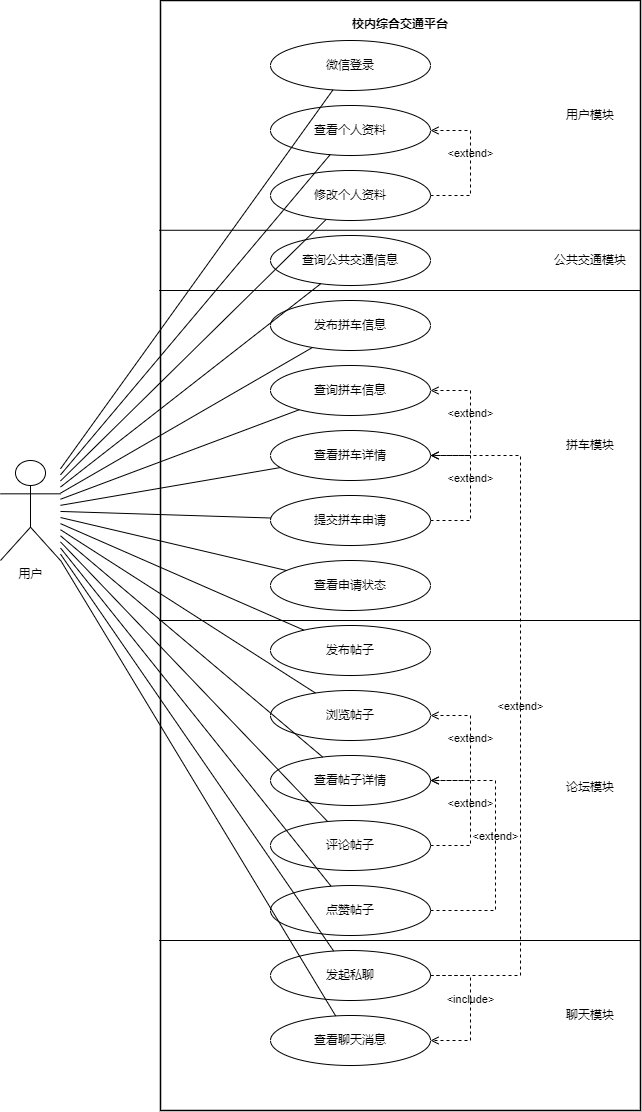
\includegraphics[width=0.62\textwidth]{figures/fig-3-1-system-usecase.png}
  \caption{系统总体用例图}
  \label{fig:overall-usecase}
\end{figure}

从\figref{fig:overall-usecase}可以看到，系统的主要交互集中在拼车、论坛、交通查询和即时沟通四部分。拼车构成主业务链，论坛和聊天则负责补充信息和协同确认。

\subsection{用户管理模块}

用户管理模块承担身份识别、资料维护和信用统计三项任务。系统采用微信授权登录完成身份初始化，避免单独设计注册流程。在用户进入系统后，需要能够稳定保存昵称、头像和联系方式等基础资料，并支持后续更新。对平台而言，这些信息不仅用于个人展示，也直接服务于拼车发布、论坛发帖和聊天会话等场景。

除基础资料外，系统还需要记录与拼车行为相关的统计项，包括信用分、完成率和迟到率。这部分数据并非独立存在，而是由拼车反馈环节持续更新，并在后续匹配过程中被再次使用。因此，用户管理模块既是身份入口，也是多个业务模块共享的基础数据来源。

\subsection{拼车服务模块}

拼车服务模块是系统的核心模块，其关键用例如\figref{fig:carpool-usecase}所示。

\begin{figure}[!htbp]
  \centering
  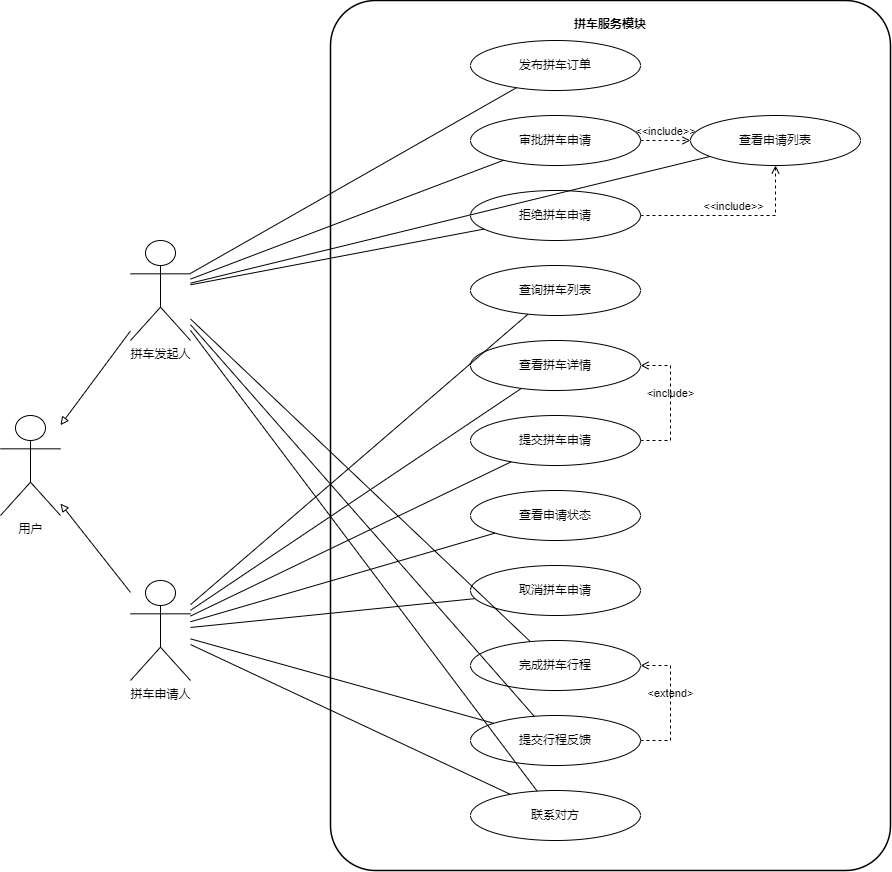
\includegraphics[width=0.74\textwidth]{figures/fig-3-2-carpool-usecase.png}
  \caption{拼车模块用例图}
  \label{fig:carpool-usecase}
\end{figure}

拼车业务首先要求系统支持结构化信息发布。用户需要提交出发地、目的地、日期、时间范围和座位信息，平台则需要对输入进行基础校验，避免地点表述混乱或时间区间无效。只有在发布环节把数据规范下来，后续筛选和排序才有可比性。

在查询阶段，系统需要支持按起点、终点、日期和时间范围进行筛选，并在筛选结果基础上给出排序。校园拼车不同于开放式社交发帖，用户通常更关心结果是否顺路、时间是否匹配以及对方是否可靠。因此，系统不仅要“查得到”，还要在满足基本约束的候选订单中给出更合理的展示顺序。

在交互阶段，系统需要支持申请加入、车主审批、撤销申请和状态查询等操作，并保证订单状态和剩余座位同步变化。行程完成后，还要允许参与人之间互评，形成后续匹配可继续使用的信用数据。由此可见，拼车模块的需求不是单个功能点的堆叠，而是一条具有状态约束的完整业务链。

\subsection{社区交流模块}

社区交流模块用于补充出行场景之外的内容互动需求。用户可以发布帖子、浏览列表、查看详情，并进行评论和点赞。对于校园平台而言，这一模块的作用不只是“增加社交性”，更重要的是为用户提供一个分享通勤经验、发布提醒信息和交流路线情况的公共空间。

该模块还需要具备基本的内容管理能力，包括图片附件处理、评论层级组织以及用户操作权限控制。例如，用户只能删除自己发布的帖子或评论，点赞操作也应避免重复记录。需求分析阶段需要把这些限制提前明确，否则后续实现容易出现内容状态与展示状态不一致的问题。

\subsection{公共交通信息模块}

公共交通信息模块负责提供校内班车和常用公交线路的查询服务。其需求相对明确：系统应能够稳定展示时刻表、线路区段和更新时间等信息，使用户在移动端快速完成浏览和判断。与拼车模块相比，该模块的交互复杂度较低，但对数据准确性和展示清晰度要求较高。

由于班车和公共交通信息更新频率相对有限，系统在需求上更强调稳定读取和清晰呈现，而不是复杂写操作。对用户而言，这一模块为拼车之外的出行选择提供了基准信息，也构成平台综合交通服务能力的重要组成部分。

\subsection{聊天与通知模块}

聊天与通知模块主要服务于拼车过程中的沟通需求。用户在查看拼车详情或收到申请结果后，往往需要进一步确认出发时间、集合地点等细节，因此系统需要支持单聊会话创建、历史消息读取和消息发送。

除即时沟通外，系统还需要在关键业务节点提供提醒，例如申请状态变化、反馈阶段开启等。通知的目的不是增加额外功能，而是减少用户遗漏关键操作的概率。聊天和通知结合后，才能把拼车从“信息发布”推进到“实际协同”。

\section{非功能需求分析}

系统的非功能需求主要体现在性能、可用性、数据管理和安全性四个方面。它们虽然不直接对应单一页面功能，但决定了平台是否能够在真实使用中稳定运行。

在性能方面，平台需要能够支撑校园场景中的集中访问，尤其是论坛列表和拼车查询等高频接口。拼车查询还涉及规则筛选和模型排序，因此响应速度不可能与简单静态页面完全相同，但应控制在用户可以接受的范围内。

在可用性方面，系统以前端小程序为主要载体，页面组织需要尽量简洁，关键流程应避免过多跳转和重复输入。对首次使用者而言，登录、查询、发布和申请等操作应当具有明确入口，避免把复杂性转移给用户。

在数据管理方面，系统需要同时处理关系型数据和文档型数据。前者强调事务与状态一致性，后者强调结构灵活和高频读写。需求分析阶段明确这一点，有助于后续数据库设计和服务边界划分。

在安全性方面，平台至少需要具备基础身份认证、权限控制和行为约束能力。拼车和聊天都涉及用户之间的直接联系，论坛又包含公开内容发布，因此隐私保护、越权操作控制和信用约束都属于必要条件，而非附加选项。

\section{可行性分析}

从技术条件看，项目采用的路线比较稳妥。微信小程序适合作为校园用户入口，Spring Boot 便于组织分层清晰的后端服务，MySQL 与 MongoDB 的组合也能覆盖系统的两类主要数据结构。随机森林排序并非唯一方案，但在样本规模有限、特征类型混合的条件下，具备较好的落地可行性。

从实现角度看，系统的业务边界相对清晰。用户、拼车、论坛、聊天和交通等模块之间既有联系，又能够分开开发和测试。项目规模能够覆盖一个完整的软件工程训练过程，同时又没有超出本科毕业设计可承受的范围。

从应用场景看，多校区通勤、班车查询和临时拼车都是真实存在的校园需求。平台建设不是为了单纯展示某种技术，而是围绕这些具体问题给出组织和实现方案。综合来看，系统在技术、实现和应用三个层面都具备继续开展设计与开发工作的条件。

\section{本章小结}

本章围绕平台的目标场景，分析了总体需求、功能需求、非功能需求和可行性。可以看到，平台要解决的并不只是“能不能查到班车”或“能不能发出拼车信息”，更重要的是把这些分散动作组织成一套能够持续运行的流程。这些结论也为后续系统设计划定了边界。
